\documentclass{article}
\usepackage{graphicx} % Required for inserting images
\usepackage[top=0.9in, bottom=1in, left=1.5in, right=1.5in]{geometry}
\usepackage[utf8]{inputenc}
\usepackage[icelandic]{babel}
\usepackage[T1]{fontenc}
\usepackage[sc]{mathpazo}
\usepackage[parfill]{parskip}
\renewcommand{\baselinestretch}{1.2}
% Tables and lists
\usepackage{booktabs,tabularx}
\usepackage{multirow}
\usepackage{enumerate}
\usepackage{adjustbox}
\usepackage{multicol}
\usepackage{xcolor}
\usepackage{algpseudocode}
\usepackage{tikz}
\usepackage{nicefrac}
\usepackage{changepage}
\usetikzlibrary{arrows, positioning, calc, graphs}

% Math
\usepackage{amsmath, amsfonts, amssymb, amsthm}
% Graphics

\usepackage{graphicx}
\usepackage{tikz}
% Code environment
\usepackage{minted}
%\usepackage{bm}
%\usepackage{siunitx}
%\usepackage{animate}
%\usepackage{hyperref}
%\usepackage{movie15}
%\usepackage{multicol}
%\usepackage{changepage}
\title{Forritunarmál Hópverkefni 6}
\author{Ragnar Björn Ingvarsson, rbi3 \\
		Daníel Snær Halldórsson, dsh11 \\
		Ólafur Sær Sigursteinsson, oss27 \\
		Máni Sverrisson, mas176 \\
		Elías Ver Bjarnason, evb17}
\tikzset{->, >=stealth', shorten >=1pt, node distance=2cm,thick, main node/.style={circle,draw,minimum size=3em}}

\begin{document}
\renewcommand\thepage{}
	
	\maketitle

	\newpage
	\setcounter{page}{1}
	\renewcommand\thepage{\arabic{page}}

	\section{}
	\begin{verbatim}
(*
Notkun: mapreduce f op u x
Fyrir: f er fall, op er tvíundaraðgerð,
       u er gildi og x er listi, x=[x1;...;xn]
Gildi: u op f(x1) op ... op f(xn)
*)
let rec mapreduce f op u x =
    match x with
      [] -> 
        u
    |
      a::b ->
        mapreduce f op (op u (f a)) b
;;
	\end{verbatim}
	\begin{center}
		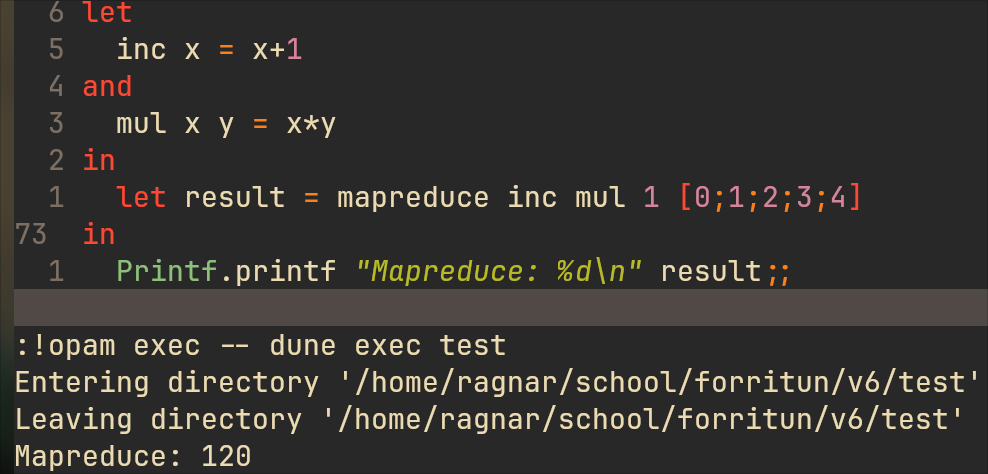
\includegraphics[scale=0.35]{mapreduce.png}
	\end{center}

	\newpage
	\section{}
	\begin{verbatim}
(*
Notkun: mapftwice f
Fyrir: f er fall sem tekur eitt viðfang af tagi 'a
Gildi: Fall sem tekur inn lista l=[l1;...;ln] af tagi 'a sem viðfang 
       og skilar [f(f(l1));...;f(f(ln))]
*)
let mapftwice f =
    (*
    Notkun: gamer x
    Fyrir: x er listi, x=[x1;...;xn]
    Gildi: [f(f(x1));...;f(f(xn))]
    *)
    let rec gamer l =
        match l with
          [] ->
            []
        |
          a::b ->
            (f (f a)) :: (gamer b)
    in 
      gamer
;;
	\end{verbatim}
	\begin{center}
		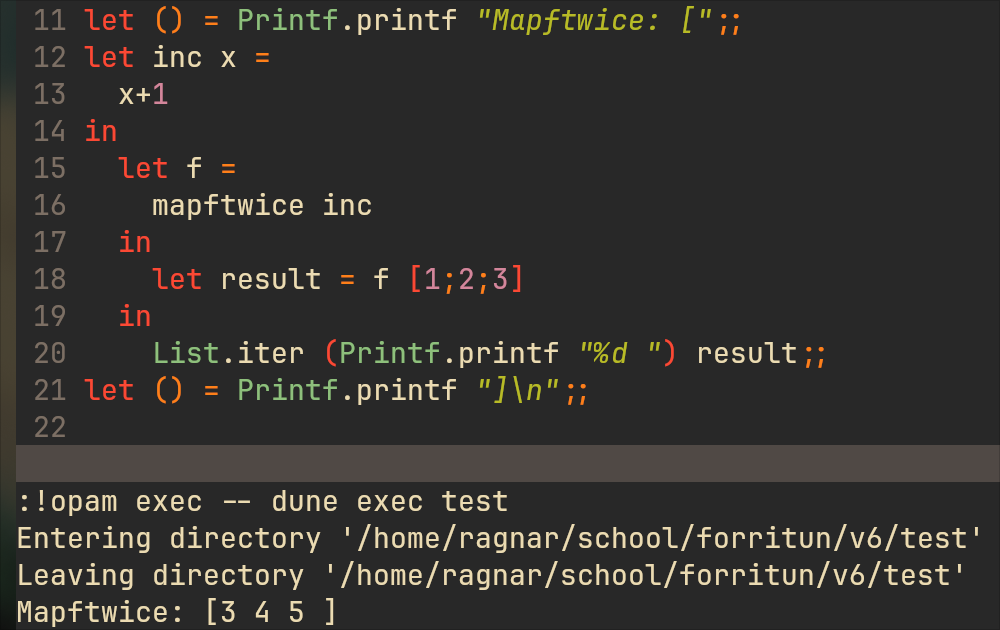
\includegraphics[scale=0.35]{mapftwice.png}
	\end{center}


\end{document}
